\subsection{Propagating solitary wave}
The propagating solitary wave tests the balancing of dispersion effects and nonlinearity for an appropriate initial condition.
On constant bathymetry, the Serre equations \cite{Serre.1953} have an analytic solitary wave solution
\begin{align}
\label{eq:Serre_sol_surface}
\xi(\bx,t)&=a \ \text{cosh}^{-2}(K(x-ct-x_0)), \\
u(\bx,t)&=c\frac{\xi(\bx,t)}{d+\xi(\bx,t)},
\end{align}
with the ratio $\frac{a}{d}=0.2$, propagation velocity $c=\sqrt{g(d+a)}$ on a constant depth $d=10 \, \text{m}$, scale factor $K=\sqrt{\left(\frac{3a}{4d^2(d+a)}\right)}$ and displacement $x_0=l/2$ on a domain of length $l=800 \, \text{m}$.
Again, we impose double periodic boundary conditions solitary wave propagating in the positive $x$-direction. The simulation time is $30$ seconds.

\subsubsection{Results of \nh\ model}
The equations \eqref{eq:nh_conti}--\eqref{eq:nh_closure} using the quadratic vertical pressure profile are equivalent to the Serre equations \cite{Serre.1953}, which is shown in  \cite{Jeschke.2016}. Using the linear vertical pressure profile, there is no equivalence to the Serre equations.
For the \nh\ model, we also need to initialize the vertical velocity, which directly follows from equation Equation \eqref{eq:nh_closure}, s.t.
\begin{align}
w&=-0.5h\partial_x u. \label{eq:nh_solit_init_w}
\end{align}
Figure \ref{fig:nh_solitarywave} compares our numerical computations with the analytical solution at the end of the simulation time.
The numerical result using the quadratic pressure profile shows a very good agreement with the analytical solution. In contrast, the application of the linear pressure profile yields a threefold mismatch arising from the inconsistency in initial conditions combined with the underlying equation system: Small amplitude waves propagate to the opposite direction, the wave height increases {because of weaker dispersion of the linear profile and trailing waves start to establish.
In \cite{StellingZijlema.2003, Walters.2005, Yamazaki.2008}, different solitary waves are computed with \nh\ models using the traditional linear vertical pressure profile. Therein, these mismatches are also visible, except that their amplitudes tend to diminish than to amplify. The reason is the application of another vertical velocity, namely $W(z)=-z\partial_x u$, so $w=-0.5(\xi-d)\partial_x u$. If the term $-d\partial_x u$ is added, the vertical velocity \eqref{eq:nh_solit_init_w} results. Hence, in \cite{StellingZijlema.2003, Walters.2005, Yamazaki.2008}, the vertical velocity is too large on the left hand side of the maximum amplitude and too small on the right hand side, which decreases the nonlinear steepening of the wave.
Their aim to compute the solitary waves was merely to show that \nh\ models produce similar results as \Bt\ models. 

\begin{figure}[htbp]
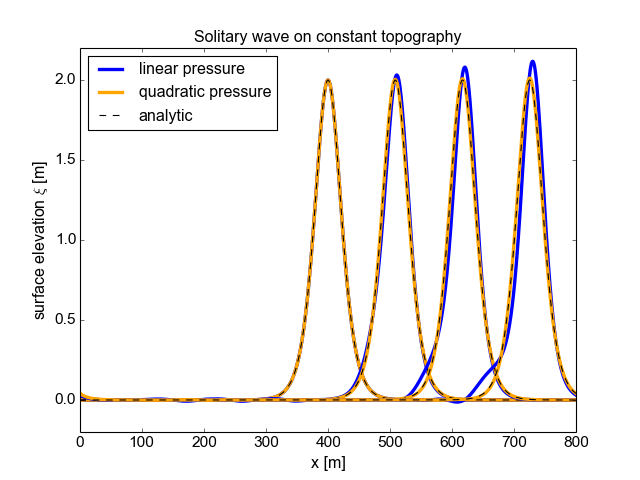
\includegraphics[width=\textwidth]{nh_solitary}
\caption{Comparison of the analytical (black) sea surface height of the
solitary wave with the simulation results of the quadratic (yellow) and linear (blue) vertical profile after a propagation time of 10, 20 and 30 seconds to the right.}
\label{fig:nh_solitarywave}
\end{figure}
